\begin{comment}
\section{Návrh a implementácia baseline riešenia}

In this chapter the design and implementation process of the baseline will be detailed. The design subsection will give a broad overview of the system architecture and explain why certain parts were chosen, while the implementation subsection will concretely detail each process used as part of the pipeline.

\subsection{Návrh baseline riešenia}

In order to help explain our reasoning for the design of the system, the following list broadly describes the general trends found in each examined system with each point being present in at least two of the solutions. 

\begin{itemize}
    \item Text concatenation of input features + text cleaning (SRCB, Anastasia, PATeam) 
    \item Usage of data augmentation (All examined solutions)
    \item Usage of LLMs for data augmentation (SRCB, MyMy, PATeam)
    \item Usage of BERT architecture for at least partial classification (SRCB, Anastasia, MyMy)
    \item Usage of fine-tuned LLMs for classification (SRCB, MyMy, PATeam)
    \item Ensemble strategies (All examined solutions)
\end{itemize}

With that in mind, our team decided that our baseline would essentially be a simplified version of the SRCB solution with three key changes:

\begin{enumerate}
    \item Data augmentation would be done with EDA \cite{wei2019eda}, not with the help of an LLM. While the team did consider using an LLM for this purpose, it was ultimately decided that it would be too advanced for a baseline solution due to the complexity, time and the subsequent costs associated with using an LLM this way.
    
    \item For training the BERT model, focal loss \cite{lin2017focal} would be used, specifically the binary variant (due to the one-vs-all setup). This is an idea borrowed from Anastasia, where the authors claim it can help with imbalanced datasets. Since EDA generally produces less diverse samples than LLM-based generation, more of the burden of handling the class imbalance falls on the loss function, which is why focal loss could prove advantageous.   
    
    \item The LLM used for the final prediction would neither be fine-tuned nor use SRCB’s label attention module, instead it would simply be given a multiple-choice prompt with the reduced label set from the BERT model.
\end{enumerate}

While this solution only effectively uses three out of the six mentioned trends, it was decided this would be a good lightweight starting point that could potentially be easily expanded to include more of the aforementioned trends. See Figure~\ref{fig:placeholder} for an overview of the proposed pipeline.
 
\begin{figure}
    \centering
    
\includegraphics[width=0.35\textwidth]{figures/floppa_placeholder.jpg}
    \caption{Placeholder}
    \label{fig:placeholder}
\end{figure}
\end{comment}

\section{Návrh a implementácia baseline riešenia}

V tejto kapitole bude podrobne opísaný proces návrhu a implementácie baseline riešenia. Podkapitola o návrhu poskytne všeobecný prehľad architektúry systému a vysvetlí, prečo boli zvolené jednotlivé časti, zatiaľ čo podkapitola o implementácii konkrétne opíše každý proces, ktorý je súčasťou pipeline.

\subsection{Návrh baseline riešenia}

Na objasnenie úvah, ktoré viedli k návrhu systému, slúži nasledujúci zoznam, ktorý všeobecne opisuje trendy nájdené v preskúmaných systémoch, pričom každý bod sa vyskytuje aspoň v dvoch riešeniach.

\begin{itemize}
    \item Spojenie vstupných atribútov do jedného textu + čistenie textu (SRCB, Anastasia, PATeam)
    \item Využitie augmentácie dát (všetky preskúmané riešenia)
    \item Využitie LLM na augmentáciu dát (SRCB, MyMy, PATeam)
    \item Využitie architektúry BERT aspoň na čiastočnú klasifikáciu (SRCB, Anastasia, MyMy)
    \item Využitie doladených LLM na klasifikáciu (SRCB, MyMy, PATeam)
    \item Ensemble stratégie (všetky skúmané riešenia)
\end{itemize}

S ohľadom na tieto trendy sa náš tím rozhodol, že baseline riešenie bude v podstate zjednodušenou verziou riešenia SRCB s tromi kľúčovými zmenami:

\begin{enumerate}
    \item Augmentácia dát bude vykonaná pomocou metódy EDA \cite{wei2019eda}, nie pomocou LLM. Hoci tím zvažoval využitie LLM na tento účel, nakoniec bolo rozhodnuté, že by to bolo pre baseline riešenie príliš pokročilé z dôvodu zložitosti, časovej náročnosti a s tým spojených nákladov na takéto využitie LLM.
    
    \item Pri trénovaní modelu BERT bude použitá stratová funkcia focal loss \cite{lin2017focal}, konkrétne jej binárna varianta (z dôvodu použitia prístupu one-vs-all). Ide o myšlienku prevzatú z riešenia Anastasia, ktorého autori tvrdia, že táto funkcia môže pomôcť pri nevyvážených datasetoch. Keďže EDA vo všeobecnosti vytvára menej rozmanité vzorky ako generovanie pomocou LLM, väčšia časť zodpovednosti za riešenie nevyváženosti tried pripadá na stratovú funkciu, a preto by sa focal loss mohla ukázať ako výhodná.
    
    \item LLM použitý na finálnu predikciu nebude doladený ani nebude využívať modul label attention z riešenia SRCB. Namiesto toho mu bude jednoducho poskytnutý prompt s výberom z viacerých možností, ktorý obsahuje zúženú množinu označení z modelu BERT.
\end{enumerate}

Hoci toto riešenie v skutočnosti využíva iba tri zo šiestich spomenutých trendov, bolo rozhodnuté, že bude vhodným a výpočtovo nenáročným začiatočným bodom, ktorý by mohol byť potenciálne jednoducho rozšírený o ďalšie zo spomenutých trendov. Pre prehľad navrhutej pipeline viď obrázok~\ref{fig:baseline_architecture}.
 
\begin{figure}
    \centering
    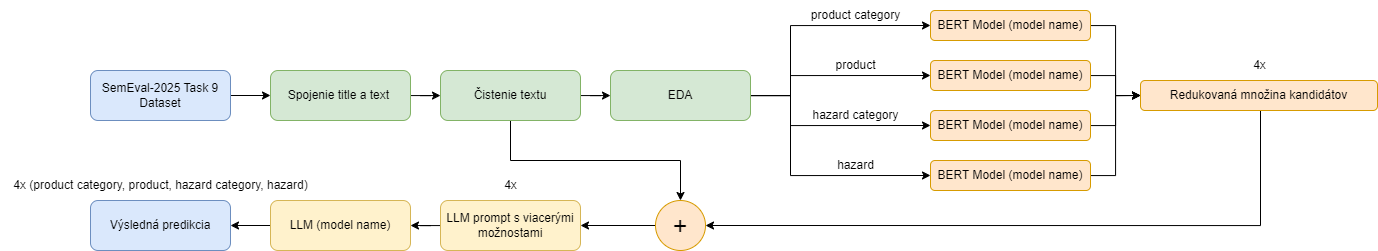
\includegraphics[width=1\textwidth]{figures/baseline_pipeline.drawio.png}
    \caption{Pipeline navrhnutého baseline riešenia.}
    \label{fig:baseline_architecture}
\end{figure}

\begin{comment}
\subsection{Implementácia baseline riešenia}

This subsection describes the individual steps of the baseline pipeline in the order in which they are performed: data preparation, data augmentation, candidate recall, LLM prediction and evaluation.

\subsubsection{Príprava dát}

As the first step, the \textit{title} and \textit{text} features of each sample are concatenated into a single text, while the remaining features (year, month, day and country) are not used. Following the SRCB solution, the resulting texts are then cleaned by normalising whitespace and line breaks, removing duplicate segments and converting all characters to lowercase. In line with SRCB, each of the four target labels (hazard category and product category for ST1, exact hazard and exact product for ST2) is treated as a separate classification problem.

\subsubsection{Augmentácia dát}

To address the class imbalance, the training set is augmented using EDA \cite{wei2019eda}. The augmentation is performed only after the data has been split, and only on the training set, to ensure that no synthetic samples end up in the validation or test sets.

Instead of augmenting the data separately for each classification problem, a single augmented dataset is created and shared by all four classifiers, with every augmented sample keeping all four labels of the sample it was created from. Since the exact product label contains by far the most underrepresented classes, it is used to drive the augmentation: every product class with fewer than (target sample count) training samples is filled up to this count by creating EDA variants of its existing samples. As each augmented sample also carries the remaining three labels, this indirectly increases their representation as well.

Each variant is created by applying the four EDA operations, namely synonym replacement, random insertion, random swap and random deletion, with (change rate) of the words in the text being modified. Since the exact hazards and products often appear literally in the text, the words corresponding to the sample's labels are protected from modification, and the \textit{title} is left unchanged, with EDA applied only to the \textit{text}. The augmentation is implemented using (EDA implementation) with a fixed random seed (seed). In total, (number of augmented samples) synthetic samples were added to the training set, increasing its size from 5\,082 to (augmented training set size) samples.

\subsubsection{Modul výberu kandidátov}

The candidate recall module reduces the set of possible labels before the final prediction by the LLM. For this purpose, (BERT model) is fine-tuned separately for each of the four classification problems, resulting in four models. Following SRCB, a one-vs-all approach is used, implemented as a multi-label classification head with one sigmoid output per label on top of the shared encoder, so that each output acts as a binary classifier for its respective label.

The models are trained using the binary variant of focal loss \cite{lin2017focal} with the parameters $\gamma$ = ($\gamma$) and $\alpha$ = ($\alpha$). The training uses the AdamW optimizer with a learning rate of (learning rate), a batch size of (batch size) and a maximum input length of (maximum length) tokens, for at most (number of epochs) epochs with early stopping based on the validation set.

After training, all labels with a predicted probability above (probability threshold) are selected as candidates. If no label exceeds this threshold, the (top-k) labels with the highest probability are selected instead, and the number of candidates is limited to at most (maximum number of candidates) in order to keep the prompts for the following step short. The resulting candidate recall, i.e.\ the proportion of samples whose correct label is among the selected candidates, was (candidate recall) on the validation set.

\subsubsection{Predikcia pomocou LLM}

The final prediction is made by an off-the-shelf LLM, (LLM), without any fine-tuning. For each sample and classification problem, a multiple-choice prompt is constructed containing a short task description, the cleaned title and text of the sample, and the candidate labels from the previous step as a numbered list, together with an instruction to answer with exactly one of the listed labels and nothing else. For ST1, (all labels / the candidate labels) are included in the prompt, since the number of categories in this sub-task is small. The candidate labels are ordered by their predicted probability from the candidate recall module, with the most probable label listed first. The full format of the prompt  is shown in Figure~\ref{fig:baseline_prompt}.

\begin{figure}
    \centering
    
\includegraphics[width=0.25\textwidth]{figures/floppa_placeholder.jpg}
    \caption{LLM prompt used to determine the final predicted lable.}
    \label{fig:baseline_prompt}
\end{figure}

To obtain deterministic outputs, the temperature is set to (temperature). The LLM's answers are then mapped to the label set: if the answer exactly matches one of the candidate labels, that label is used; otherwise, the most similar label is selected using (string matching method). If no sufficiently similar label is found, the candidate with the highest probability from the candidate recall module is used as a fallback.
\end{comment}

\subsection{Implementácia baseline riešenia}

Táto podkapitola opisuje jednotlivé kroky pipeline baseline riešenia v poradí, v akom sú vykonávané: príprava dát, augmentácia dát, výber kandidátov, a výsledná predikcia pomocou LLM.

\subsubsection{Príprava dát}

V prvom kroku sú atribúty \textit{title} a \textit{text} každej vzorky spojené do jedného textu, pričom zvyšné atribúty (\textit{year}, \textit{month}, \textit{day} a \textit{country}) nie sú použité. Podľa vzoru riešenia SRCB sú výsledné texty následne vyčistené normalizáciou bielych znakov a zalomení riadkov, odstránením duplicitných úsekov a prevodom všetkých znakov na malé písmená. V súlade s riešením SRCB je každé zo štyroch cieľových označení (kategória hazardu a kategória produktu pre ST1, konkrétny hazard a konkrétny produkt pre ST2) považované za samostatný klasifikačný problém.

\subsubsection{Augmentácia dát}

Na riešenie nevyváženosti tried je trénovacia množina augmentovaná pomocou metódy EDA \cite{wei2019eda}. Augmentácia je vykonaná až po rozdelení dát a iba na trénovacej množine, aby sa zabezpečilo, že sa žiadne syntetické vzorky nedostanú do validačnej ani testovacej množiny.

Namiesto samostatnej augmentácie dát pre každý klasifikačný problém je vytvorený jeden augmentovaný dataset, ktorý je zdieľaný všetkými štyrmi klasifikátormi, pričom každá augmentovaná vzorka si zachováva všetky štyri označenia vzorky, z ktorej bola vytvorená. Keďže označenie konkrétneho produktu obsahuje zďaleka najviac málo zastúpených tried, augmentácia je riadená práve ním: každá trieda produktu s menej ako (target sample count) trénovacími vzorkami je doplnená na tento počet vytvorením EDA variantov jej existujúcich vzoriek. Keďže každá augmentovaná vzorka nesie aj zvyšné tri označenia, nepriamo sa tým zvyšuje aj ich zastúpenie.

Každý variant je vytvorený aplikovaním štyroch operácií EDA, konkrétne nahradenia synonymom, náhodného vloženia, náhodnej zámeny a náhodného vymazania, pričom je upravených (change rate) slov v texte. Keďže konkrétne hazardy a produkty sa v texte často vyskytujú doslovne, slová zodpovedajúce označeniam vzorky sú chránené pred úpravou a \textit{title} zostáva nezmenený, pričom EDA je aplikovaná iba na \textit{text}. Augmentácia je implementovaná pomocou (EDA implementation) s pevne nastaveným náhodným seedom (seed). Celkovo bolo do trénovacej množiny pridaných (number of augmented samples) syntetických vzoriek, čím sa jej veľkosť zvýšila z 5\,082 na (augmented training set size) vzoriek.

\subsubsection{Modul výberu kandidátov}

Modul výberu kandidátov zužuje množinu možných označení pred finálnou predikciou pomocou LLM. Na tento účel je model (BERT model) doladený samostatne pre každý zo štyroch klasifikačných problémov, výsledkom čoho sú štyri modely. Podľa vzoru riešenia SRCB je použitý prístup one-vs-all, implementovaný ako multi-label klasifikačná hlava s jedným sigmoidovým výstupom pre každé označenie nad zdieľaným enkodérom, takže každý výstup funguje ako binárny klasifikátor pre príslušné označenie.

Modely sú trénované pomocou binárnej varianty focal loss \cite{lin2017focal} s parametrami $\gamma$ = ($\gamma$) a $\alpha$ = ($\alpha$). Trénovanie využíva optimalizátor AdamW s rýchlosťou učenia (learning rate), veľkosťou dávky (batch size) a maximálnou dĺžkou vstupu (maximum length) tokenov, pričom trvá najviac (number of epochs) epoch s predčasným zastavením (early stopping) na základe validačnej množiny.

Po natrénovaní sú ako kandidáti vybrané všetky označenia s predikovanou pravdepodobnosťou vyššou ako (probability threshold). Ak žiadne označenie túto hranicu neprekročí, namiesto toho je vybraných (top-k) označení s najvyššou pravdepodobnosťou, pričom počet kandidátov je obmedzený na najviac (maximum number of candidates), aby prompty pre nasledujúci krok zostali krátke. Výsledný recall kandidátov, t.\,j. podiel vzoriek, ktorých správne označenie sa nachádza medzi vybranými kandidátmi, dosiahol na validačnej množine hodnotu (candidate recall).

\subsubsection{Predikcia pomocou LLM}

Finálna predikcia je vykonaná bežne dostupným LLM (LLM) bez akéhokoľvek doladenia. Pre každú vzorku a klasifikačný problém je zostavený prompt s výberom z viacerých možností, ktorý obsahuje krátky opis úlohy, vyčistený nadpis a text vzorky a kandidátske označenia z predchádzajúceho kroku vo forme číslovaného zoznamu, spolu s inštrukciou odpovedať práve jedným z uvedených označení a ničím iným. Pre ST1 sú v prompte zahrnuté (all labels / the candidate labels), keďže počet kategórií v tejto podúlohe je malý. Kandidátske označenia sú zoradené podľa predikovanej pravdepodobnosti z modulu výberu kandidátov, pričom najpravdepodobnejšie označenie je uvedené ako prvé. Úplný formát promptu je zobrazený na obrázku~\ref{fig:baseline_prompt}.

\begin{figure}
    \centering
    
\includegraphics[width=0.25\textwidth]{figures/floppa_placeholder.jpg}
    \caption{Prompt pre LLM použitý na určenie výsledného predikovaného označenia.}
    \label{fig:baseline_prompt}
\end{figure}

Na získanie deterministických výstupov je teplota nastavená na (temperature). Odpovede LLM sú následne priradené k množine označení: ak sa odpoveď presne zhoduje s jedným z kandidátskych označení, je použité toto označenie, v opačnom prípade je pomocou (string matching method) vybrané najpodobnejšie označenie. Ak nie je nájdené dostatočne podobné označenie, ako záložné riešenie je použitý kandidát s najvyššou pravdepodobnosťou z modulu výberu kandidátov.

\begin{comment}
\section{Výsledky baseline riešenia}

Our solution achieved a (score) placing us (ST1 placement) for ST1 and (score) placing us (ST2 placement) for ST2. See Figure~\ref{fig:baseline_cm} for the resulting confusion matrices.

\begin{figure}
    \centering
    
\includegraphics[width=0.25\textwidth]{figures/floppa_placeholder.jpg}
    \caption{Confusion matrices using our baseline for ST1 and ST2}
    \label{fig:baseline_cm}
\end{figure}

\section{Použitie agentov a LLM mimo riešenia}

A LLM specifically Claude Opus 5.5 was used during the development of this project for:

\begin{itemize}
    \item Text critique (e.q. "Here is my section on MyMy, what do you think ? Is there anything that should be added ?")
    \item Clarification of concepts (e,q "Was the pipeline for both subtasks the same ?", "How is the sample and relevant documents combined into a prompt, are they just attached or are they somehow embedded together ?")
    \item Image extraction from documents (e.q "Can you extract the LLM prediction module image from page 999 for me ?")
    \item Language translation
\end{itemize}
\end{comment}

\section{Výsledky baseline riešenia}

Naše riešenie dosiahlo v ST1 skóre (score), čím sa umiestnilo na (ST1 placement) mieste, a v ST2 skóre (score), čím sa umiestnilo na (ST2 placement) mieste. Pre výsledné konfúzné matice pre ST1 viď obrázok~\ref{fig:baseline_cm_product},~\ref{fig:baseline_cm_hazard} (ST2 má príliš veľa možných označení pre zmysluplnú vizualizáciu).

\begin{figure}
    \centering
    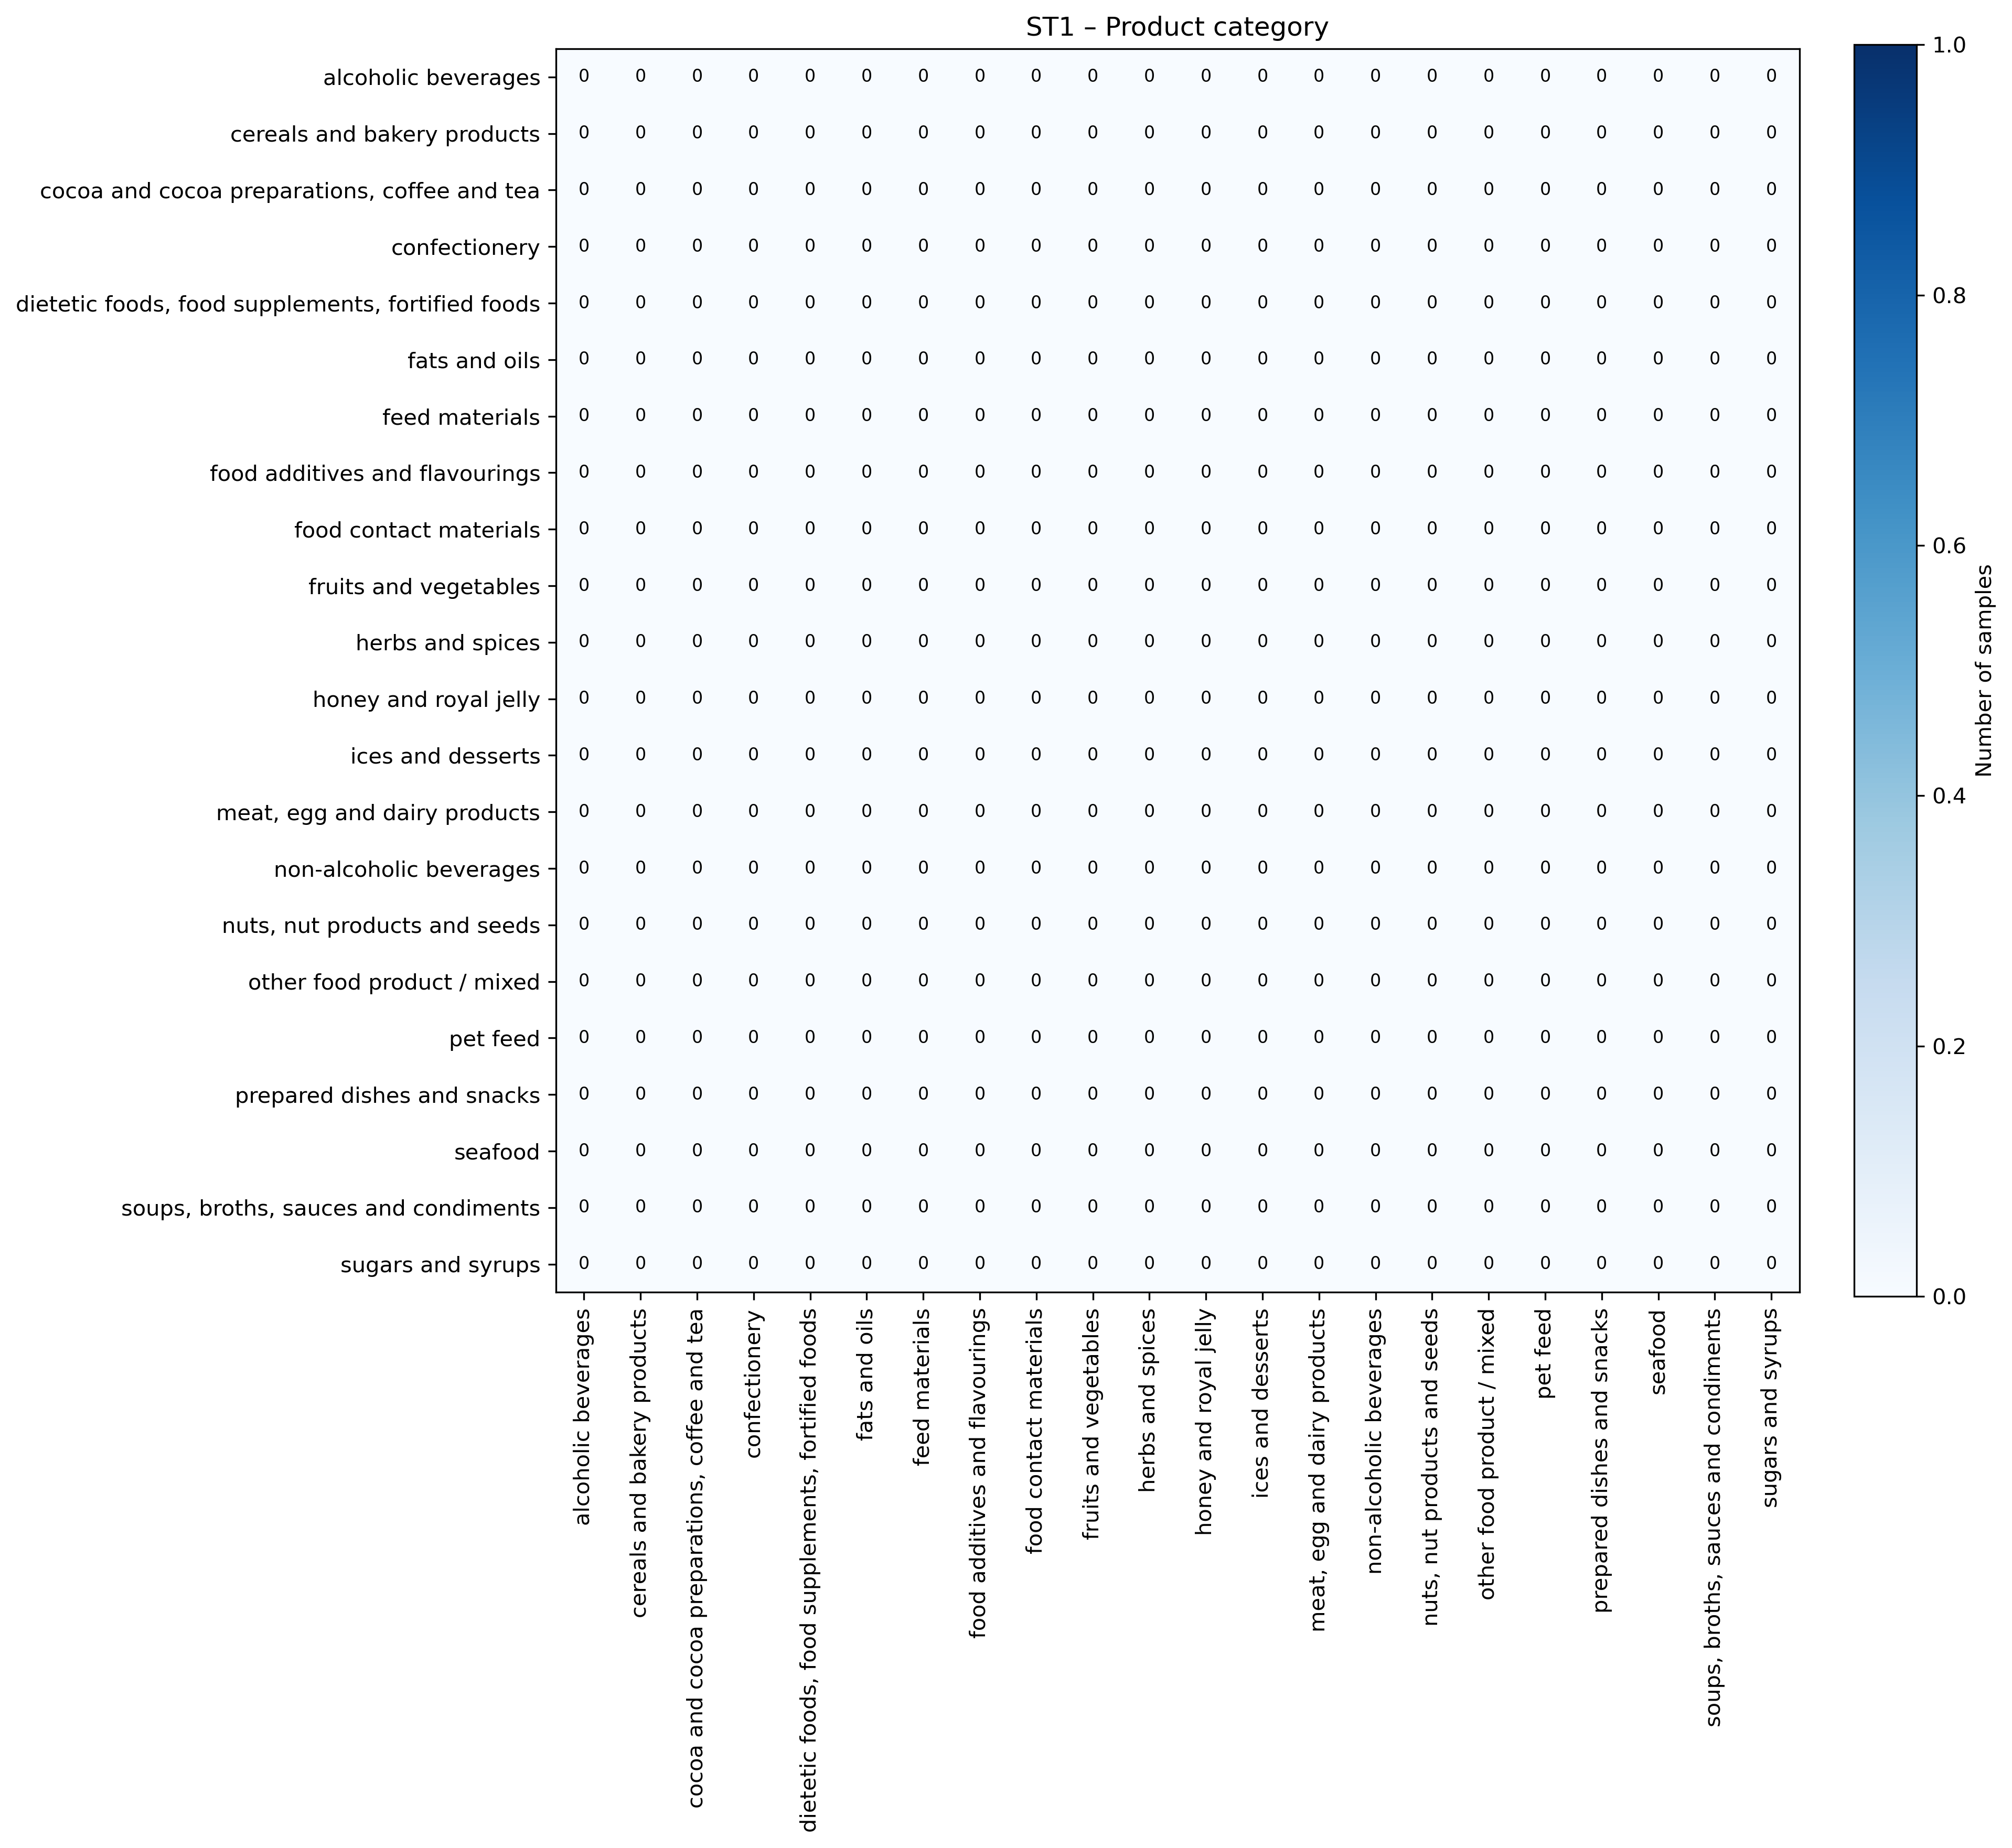
\includegraphics[width=0.95\textwidth]{figures/st1_confusion_product.png}
    \caption{Konfúzna matica pre baseline riešenie pre ST1 - product.}
    \label{fig:baseline_cm_product}
\end{figure}

\begin{figure}
    \centering
    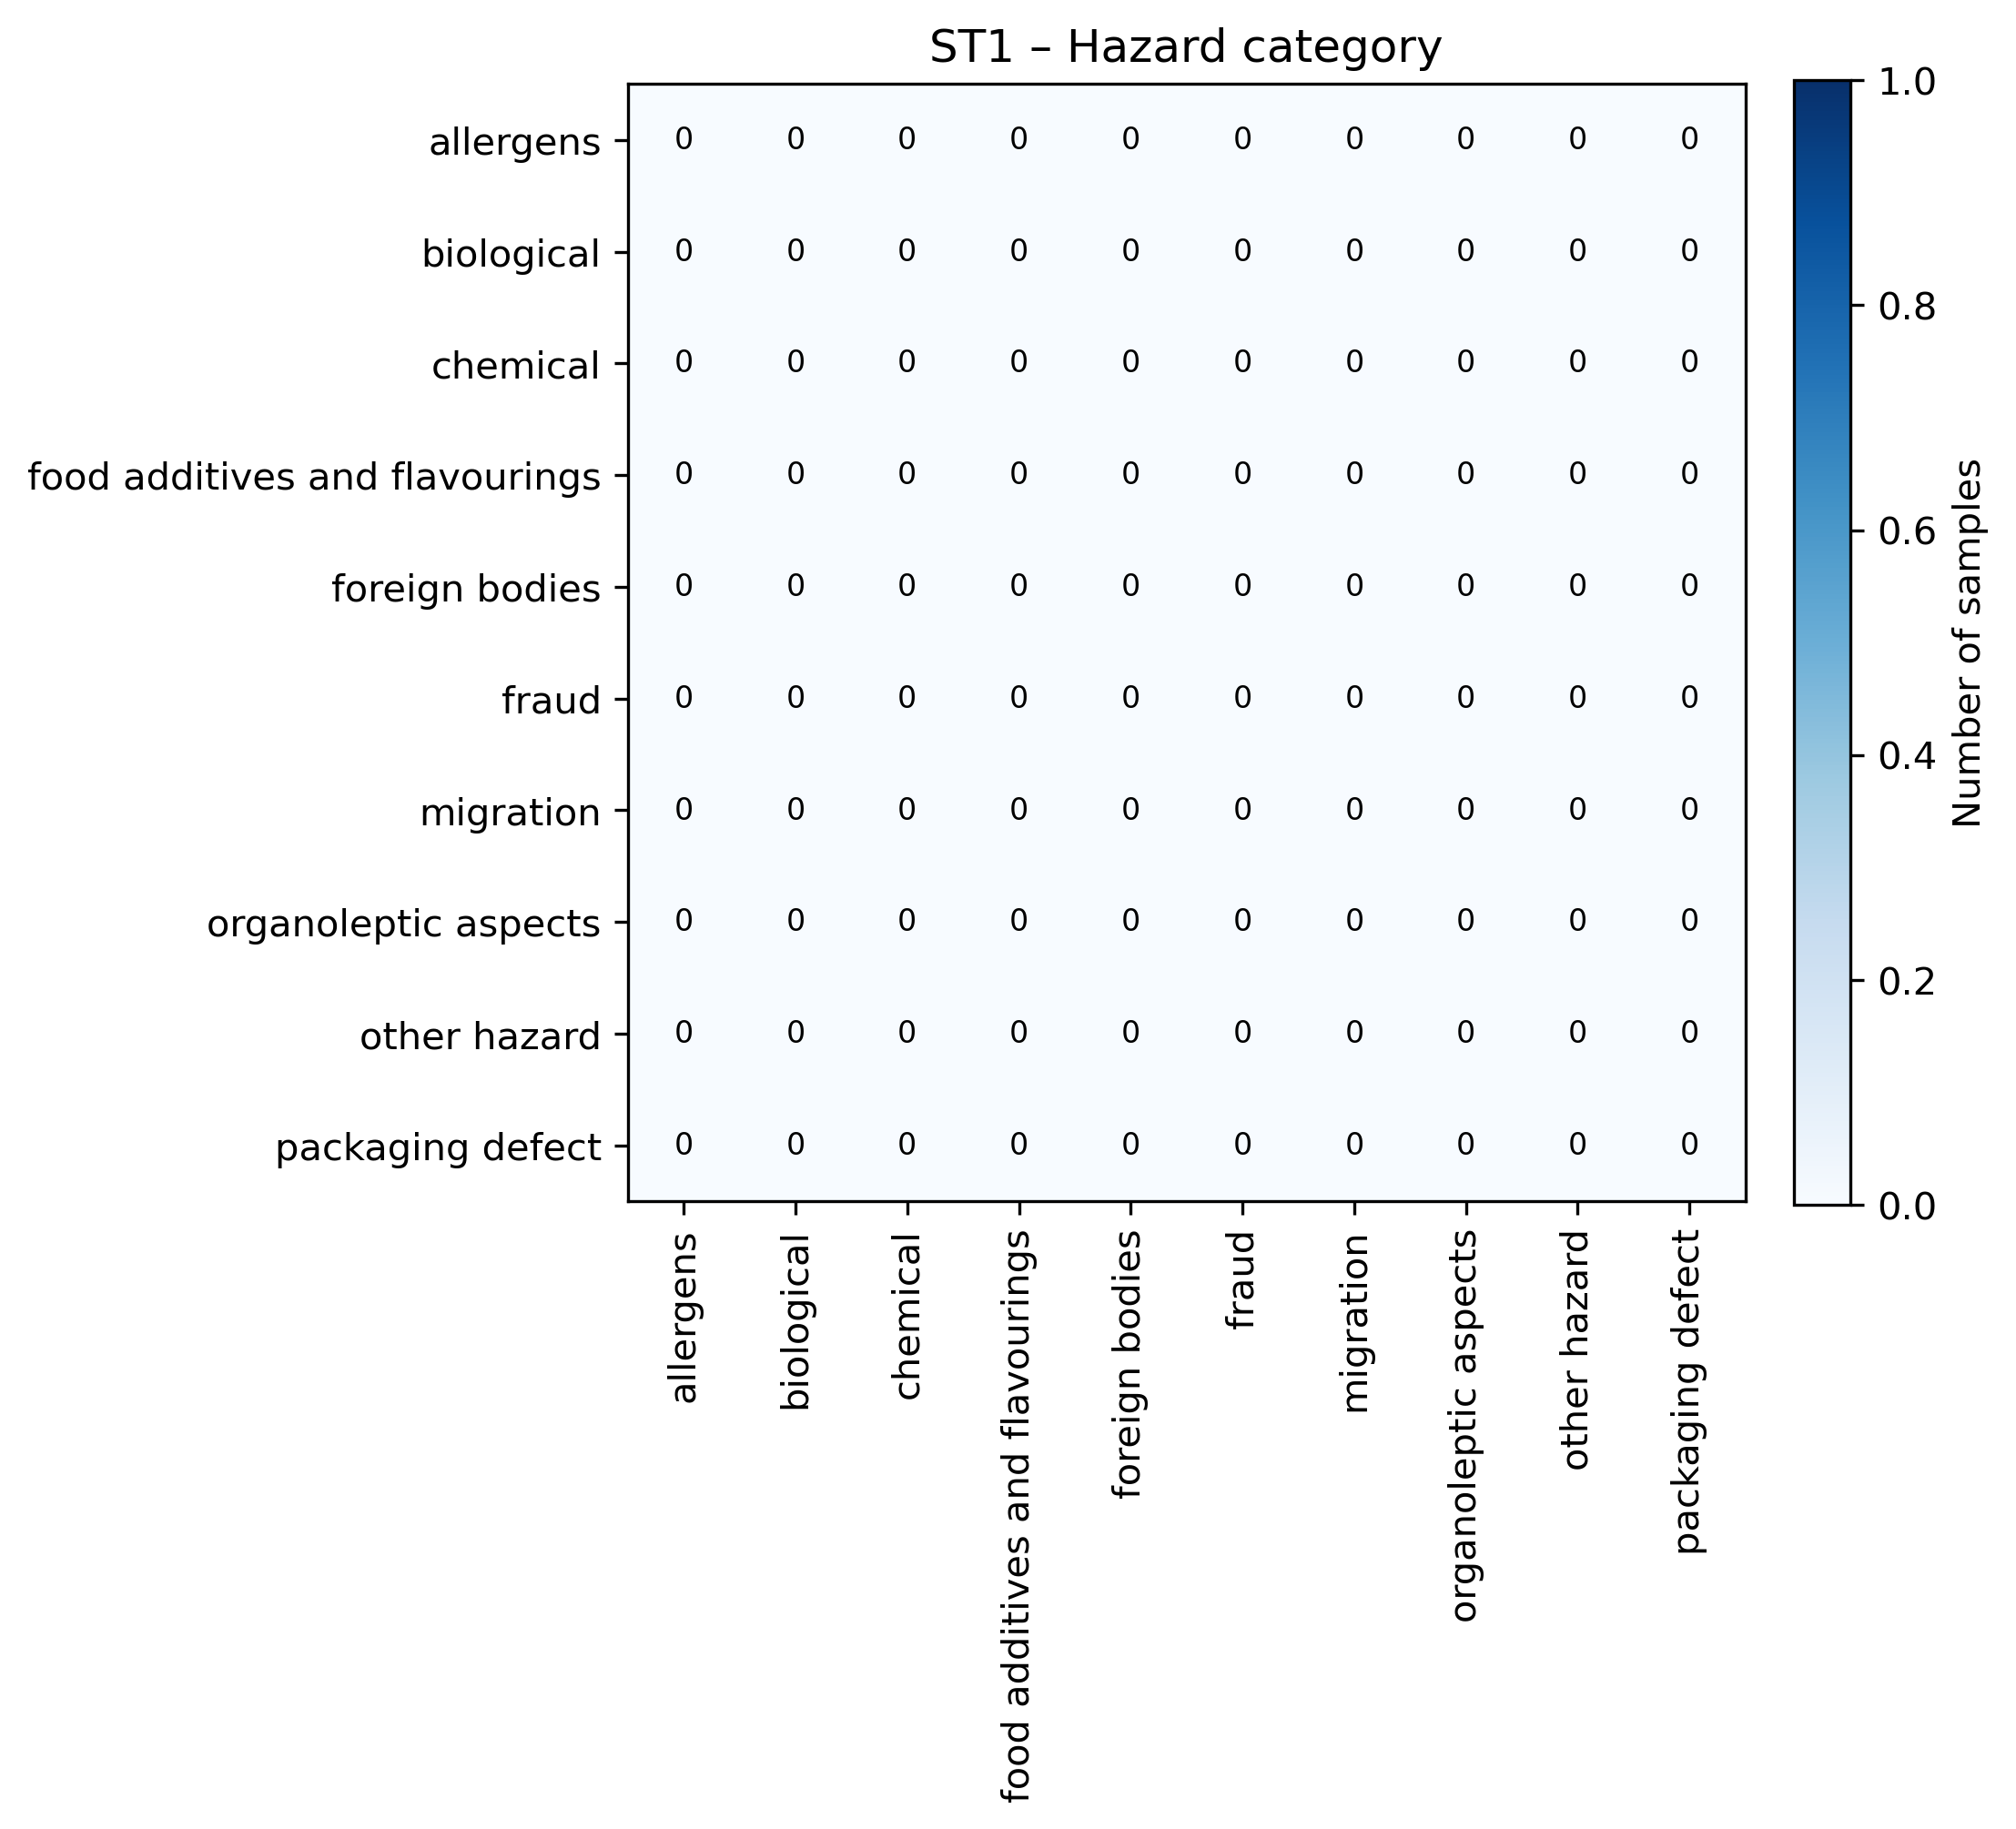
\includegraphics[width=0.95\textwidth]{figures/st1_confusion_hazard.png}
    \caption{Konfúzna matica pre baseline riešenie pre ST1 - hazard.}
    \label{fig:baseline_cm_hazard}
\end{figure}

\section{Použitie agentov a LLM mimo riešenia}

Počas vývoja tohto projektu bol použitý LLM, konkrétne Claude Opus 5.5, na:

\begin{itemize}
    \item Kritiku textu (napr. \uv{Here is my section on MyMy, what do you think? Is there anything that should be added?})
    \item Objasnenie pojmov (napr. \uv{Was the pipeline for both subtasks the same?}, \uv{How is the sample and relevant documents combined into a prompt, are they just attached or are they somehow embedded together?})
    \item Extrakciu obrázkov z dokumentov (napr. \uv{Can you extract the LLM prediction module image from page 999 for me?})
    \item Preklad textu
\end{itemize}